 \chapter{Operações Numéricas}

 Antes de tratar das operações numéricas e algébricas, vale ressaltar que quando estamos resolvendo uma expressão numérica ou uma expressão algébrica temos vários cálculos para serem feitos sucessivamente, e para tal precisamos obedecer uma ordem de prioridades que é a seguinte:

\begin{multicols}{2}
Resolva em:
\begin{itemize}
\item 1º lugar: raízes e potências;
\item 2º lugar: multiplicação e divisão;
\item 3º lugar: adição e subtração.
\end{itemize}

Priorize cálculos em:
\begin{itemize}
\item 1º lugar: parênteses $($ $)$;
\item 2º lugar: colchetes $[$ $]$;
\item 3º lugar: chaves $\{$ $\}$.
\end{itemize}
\end{multicols}

 \section{Operações em \texorpdfstring{$\Z$}{Z}}

 Ao operar neste conjunto numérico precisamos lidar com os números negativos e para isso precisamos dominar os jogos de sinais envolvidos nestas operações, então vamos ver alguns exemplos de operações neste conjunto para entender como lidar com os números negativos.

 \textbf{Adição de números inteiros}

 \begin{itemize}
  \item Na adição de números inteiros com o mesmo sinal, some os números e conserve o sinal;
  \item Na adição de números inteiros com sinais diferentes, subtraia os números e conserve o sinal do maior.
 \end{itemize}

  \begin{enumerate}[1)]
   \item $123 + 7= 130$
   \item $123 - 7= 116$
   \item $-123 + 7 = -116$
   \item $-123 - 7 = -130$
 \end{enumerate}

 \textbf{Multiplicação e divisão de números inteiros}

  \begin{itemize}
   \item Na multiplicação e divisão de números inteiros com o mesmo sinal o resultado é sempre positivo.
   \item Na multiplicação e divisão de números inteiros com o sinais diferentes o resultado é sempre negativo.
  \end{itemize}

  \begin{multicols}{2}
  \begin{enumerate}[1)]
   \item $8 \cdot 20= 160$
   \item $8 \cdot (-20)= -160$
   \item $-8 \cdot 20= -160$
   \item $(-8) \cdot (-20)= 160$
   \item $45 \div 5= 9$
   \item $45 \div (-5)= -9$
   \item $(-45) \div 5= -9$
   \item $(-45) \div (-5)= 9$
  \end{enumerate}
  \end{multicols}



 \section{Operações em \texorpdfstring{$\Q$}{Q}}

 As operações no conjunto dos números Racionais envolvem em particular as operações com frações que possuem algumas particularidades por isso façamos uma rápida retomada destas operações.

 \vskip0.3cm

 \colorbox{azul}{
 \begin{minipage}{0.9\linewidth}
 \begin{center}
  \textbf{Soma:} Dados $x, y, a, b \in \Z$ com $a, b \neq 0$ temos:
 \[\frac{x}{a} + \frac{y}{a}= \frac{x+y}{a} \, \text{ ou}, \ \
  \frac{x}{a} + \frac{y}{b}= \frac{xb + ya}{ab} \]
 \end{center}
 \end{minipage}}

 \vskip0.3cm

 \colorbox{azul}{
 \begin{minipage}{0.9\linewidth}
 \begin{center}
  \textbf{Subtração:} Dados $x, y, a, b \in \Z$ com $a, b \neq 0$ temos:
 \[\frac{x}{a} - \frac{y}{a}= \frac{x-y}{a} \, \text{ ou}, \ \
 \frac{x}{a} - \frac{y}{b}= \frac{xb - ya}{ab} \]
 \end{center}
 \end{minipage}}

 \vskip0.3cm

 \begin{exem}
  \textbf{Soma e subtração de frações com mesmo denominador:}

   Quando os denominadores das frações são iguais, mantemos o denominador e operamos os numeradores.
    \vskip0.3cm
   \[\frac{3}{5} + \frac{1}{5}= \frac{3+1}{5}= \frac{4}{5} .\]
    \vskip0.3cm
   \[\frac{3}{5} - \frac{1}{5}= \frac{3-1}{5}= \frac{2}{5} .\]
 \end{exem}

 \begin{exem}
 \textbf{Soma e subtração de frações com denominadores diferentes:}

   Quando os denominadores das frações são diferentes podemos simplesmente multiplicar os denominadores ou calcular o mínimo múltiplo comum entre eles (MMC), a vantagem da segunda opção é que o MMC é menor ou igual ao produto, como podemos ver no exemplo:
    \vskip0.3cm
   \[\frac{2}{4} + \frac{3}{10}= \frac{10 \cdot 2 + 4 \cdot 3}{4 \cdot 10}= \frac{20 + 12}{40}= \frac{32}{40}= \frac{4}{5} .\]
    \vskip0.3cm
   \[\frac{2}{4} - \frac{3}{10}= \frac{10 \cdot 2 - 4 \cdot 3}{4 \cdot 10}= \frac{20 - 12}{40}= \frac{8}{40}= \frac{1}{5} .\]
    \vskip0.3cm
   Observamos que o $MMC(4, 10)= 20$, assim,
    \vskip0.3cm
   \[\frac{2}{4} + \frac{3}{10}= \frac{5 \cdot 2 + 2 \cdot 3}{20}= \frac{10+6}{20}= \frac{16}{20}=\frac{4}{5} .\]
    \vskip0.3cm
   \[\frac{2}{4} - \frac{3}{10}= \frac{5 \cdot 2 - 2 \cdot 3}{20}= \frac{10 - 6}{20}= \frac{4}{20}=\frac{1}{5} .\]
 \end{exem}


 \vskip0.5cm

 \colorbox{azul}{
 \begin{minipage}{0.9\linewidth}
 \begin{center}
  \textbf{Multiplicação:} Dados $a, b, c, d \in \Z$ com $b, d \neq 0$ temos:
 \[\frac{a}{b} \cdot \frac{c}{d}= \frac{a \cdot c}{b \cdot d} \]
 \end{center}
 \end{minipage}}

 \vskip0.3cm
 \begin{exem}
  \textbf{Multiplicação de fração:} na multiplicação devemos multiplicar numerador por numerador e denominador por denominador.
   \[\frac{2}{3} \cdot \frac{6}{4}= \frac{2 \cdot 6}{3 \cdot 4}= \frac{12}{12}= 1 \]
   \[2 \cdot \frac{5}{3}= \frac{2 \cdot 5}{3}= \frac{10}{3}\]
 \end{exem}

 \vskip0.3cm

 \colorbox{azul}{
 \begin{minipage}{0.9\linewidth}
 \begin{center}
  \textbf{Divisão:} Dados $a, b, c, d \in \Z$ com $b, c, d \neq 0$ temos:
 \[\frac{a}{b} \div \frac{c}{d}= \frac{a}{b} \cdot \frac{d}{c} \]
 \end{center}
 \end{minipage}}

 \vskip0.3cm
 \begin{exem}
  \textbf{Divisão de fração:} na divisão conservamos a primeira fração e multiplicamos pelo inverso da segunda.
   \[\frac{2}{3} \div \frac{1}{6}= \frac{2}{3} \cdot \frac{6}{1}= \frac{2 \cdot 6}{3 \cdot 1}= \frac{12}{3}= 4 \]
   \[\frac{4}{\left(\frac{2}{3}\right)}= \frac{4}{1} \cdot \frac{3}{2}= \frac{12}{2}=6\]
 \end{exem}


 \vskip0.3cm


 \section{Potenciação}

  \vskip0.3cm

 \textbf{Potência}

 \vskip0.3cm

 \colorbox{azul}{
 \begin{minipage}{0.9\linewidth}
 \begin{center}
  Dados dois números $a \in \R$ e $b \in \N$ definimos:
 \[a^b= \underbrace{a \cdot a \cdot \cdots \cdot a}_{b \text{ vezes}} .\]
  Dizemos que $a$ é a base da potência e $b$ o expoente. Lê-se: $a$ elevado a $b$.
 \end{center}
 \end{minipage}}

 \vskip0.3cm

 \begin{exem}
 Observe que neste caso o expoente é um número natural, e portanto positivo, como por exemplo:

  $2^3= 2 \cdot 2 \cdot 2= 8$;

  $2^4=2 \cdot 2 \cdot 2 \cdot  2= 16$;

  $3^2= 3 \cdot 3= 9$;

  $5^3= 5 \cdot 5 \cdot 5= 125$.

  Este é o único caso em que temos a potência definida, se tivermos qualquer outro número no expoente precisamos fazer recair nesta situação.
 \end{exem}


 \vskip0.3cm

 \colorbox{azul}{
 \begin{minipage}{0.9\linewidth}
 \begin{center}
   Dados dois números $a \in \R$ e $b \in \Z$ definimos:
 \[a^b= \underbrace{a \cdot a \cdot \cdots \cdot a}_{b \text{ vezes}}, \text{ para } b\geq0, \text{ esta situação está inclusa no caso anterior};\]
 \[a^{-b}= \frac{1}{a^b}= \underbrace{\frac{1}{a} \cdot \frac{1}{a} \cdot \cdots \cdot \frac{1}{a}}_{b \text{ vezes}}, \text{ para } b>0 ;\]
 \[\frac{1}{a^{-b}}= a^b, \text{ para } b>0;\]
 \end{center}
 \end{minipage}}

 \vskip0.3cm

 \begin{exem}
 Vejamos agora alguns exemplos em que o expoente é um número negativo:
 \begin{eqnarray*}
  2^{-1}= \frac{1}{2^{1}}= \frac{1}{2}; \\
  2^{-3}= \frac{1}{2^3}= \frac{1}{8}; \\
  \frac{1}{3^{-2}}= 3^2= 3 \cdot 3= 9; \\
  \left( \frac{8}{22} \right)^{-2}= \left( \frac{22}{8} \right)^{2}= \frac{22}{8} \cdot \frac{22}{8}= \frac{484}{64}.
 \end{eqnarray*}
 Note que em todos os exemplos acima o que fizemos foi "inverter" a fração, e com isso deixamos os expoentes positivos, e então basta aplicar a definição de potência.

 \end{exem}

 \vskip0.3cm

 \textbf{Raiz}

 \vskip0.3cm

 \colorbox{azul}{
 \begin{minipage}{0.9\linewidth}
 \begin{center}
  Dados dois números $a \in \R$ e $b \in \Q$, logo $b= \frac{m}{n}$ para $n \neq 0$, definimos:
 \[a^b= a^{\frac{m}{n}}= \sqrt[n]{a^m}, \text{ para } b>0 ;\]
 \[a^{-b}= \frac{1}{a^{\frac{m}{n}}}= \frac{1}{\sqrt[n]{a^m}},  \text{ para } b>0.\]
 \end{center}
 \end{minipage}}

 \vskip0.3cm

 \begin{exem}
  Vejamos agora alguns exemplos de potência com expoente sendo um número racional ($b \in \mathbb{Q}$):
  \begin{eqnarray*}
   4^{\frac{1}{2}}= \sqrt{4}= 2 \\
   8^{\frac{1}{3}}= \sqrt[3]{8^1}= \sqrt[3]{2^{3}}= 2 \\
   27^{\frac{2}{6}}= \sqrt[6]{27^2}= \sqrt[6]{729}= \sqrt[6]{3^6}= 3\\
   9^{-\frac{1}{2}}= \frac{1}{9^{\frac{1}{2}}}= \frac{1}{\sqrt{9}}= \frac{1}{3} \\
   \left(\frac{4}{9}\right)^{-\frac{1}{2}}= \left(\frac{9}{4}\right)^{\frac{1}{2}}= \sqrt{\left(\frac{9}{4}\right)}=\frac{\sqrt{9}}{\sqrt{4}}= \frac{3}{2} \\
   \frac{2}{3^{-2}}= 2 \cdot \frac{1}{3^{-2}}= 2 \cdot 3^{2}= 2 \cdot 9= 18
  \end{eqnarray*}

 \end{exem}


 \vskip0.3cm

 \colorbox{amarelo}{
 \begin{minipage}{0.9\linewidth}
 \begin{center}
 Aqui é importante observar que:
 \begin{align*}
 & \nexists 0^0 & & a^1= a, \forall a \in \R & & a^0= 1, \forall a \in \R & & 1^a= 1, \forall a \in \R
 \end{align*}
 \end{center}
 \end{minipage}}

 Além disso a operação de potenciação satisfaz as seguintes propriedades:

  \begin{table}[H]
 \centering
 \begin{tabular}{|c|c|} \hline
 $a^m \cdot a^n= a^{m + n}$ & $a^m \div a^n= a^{m - n}$ \\ \hline
 $(a^m)^n= a^{m \cdot n}$ & $(a \cdot b)^n= a^n \cdot b^n$ \\ \hline
 $\left(\frac{a}{b}\right)^n= \frac{a^n}{b^n}$ & $a^{-n}= \frac{1}{a^n}$ $(a \neq 0)$ \\ \hline
 $\left(\frac{a}{b} \right)^{-n}= \left(\frac{b}{a} \right)^{n}$ & $a^{\frac{m}{n}}= \sqrt[n]{a^m}$ \\\hline
 \end{tabular}
 \end{table}

 \chapter{Operações Algébricas}

 Expressões algébricas são expressões matemáticas que envolvem números, letras e operações.

 Como por exemplo:

 \begin{eqnarray*}
  2x=4,\\
  x^2+1=0,\\
  x(x+3)=5,\\
  2x+3y=17,\\
  x^2 + 2y + 3z -4= 52, \\
  \frac{14x + 8y}{2x}= 3, \\
  \frac{2}{5}x^3 + 3\sqrt{x^4}= 67, \\
  5x(x+3)-4x(2-x)=7.
 \end{eqnarray*}

 Nestas expressões as letras que aparecem são chamadas de \textbf{variáveis}, e os números que aparecem multiplicando uma letra são chamados de \textbf{coeficientes}.

 As expressões algébricas são utilizadas dentre outras coisas, para descrever uma situação problema na qual não conhecemos todos os valores envolvidos, representar uma fórmula, ou expressar uma equação. Devido a sua importância nas exatas precisamos compreender como se comportam as operações presentes nas expressões algébricas, em outras palavras, como fazer contas com letras.

 \vskip0.3cm

 \textbf{Adição e subtração}

 Podemos somar somente letras iguais e com mesmo expoente. Como por exemplo:

 \begin{itemize}
  \item $2x + x= (2+1)x= 3x$
  \item $x^2 - 3x^2= (1-3)x^2= -2x^2$
  \item $2x + y + 5x^2 + 7y - 3x= 5x^2 + (2-3)x + (1+7)y= 5x^2 - 1x + 8y$
  \item $3(x+ 4y-2)= 3x + 3.4y - 3.2= 3x + 12y - 6$
 \end{itemize}

  \vskip0.3cm

 \textbf{Multiplicação}

 Na multiplicação devemos sempre multiplicar coeficiente por coeficiente e letra por letra. Sendo que no caso das letras serem iguais, devemos manter a letra e somar seus expoentes, e no caso das letras serem diferentes apenas fazemos a associação das duas letras. Como mostram os seguintes exemplos:

  \begin{itemize}
   \item $x \cdot x = x^{1+1}= x^2$
   \item $x \cdot x^2= x^{1+2}= x^3$
   \item $x \cdot 2y= (1 \cdot 2)xy= 2xy$
   \item $3x \cdot 2x^2y= (3 \cdot 2)x^{1+2}y= 6x^3y$
   \item $4x^4 \cdot \frac{1}{2}x^{-2}= (4 \cdot \frac{1}{2})x^{4-2}= 2x^2$
   \item $(x - 1) \cdot (x - 2)= x(x-2) - 1(x-2)= x^2 -2x -x +2= x^2 - 3x + 2$
  \end{itemize}

  \vskip0.3cm

   \textbf{Divisão}

   Na divisão devemos sempre dividir coeficiente por coeficiente e letra por letra. Sendo que no caso das letras serem iguais, devemos manter a letra e subtrair seus expoentes, e no caso das letras serem diferentes apenas fazemos a associação das duas letras. Como mostram os seguintes exemplos:

  \begin{itemize}
   \item $x \div x= x^{1-1}= x^0= 1$
   \item $x \div x^2= x^{1-2}= x^{-1}= \frac{1}{x}$
   \item $2y \div x= 2\frac{y}{x}$
   \item $4y^3 \div 2y^2= \frac{4}{2} \cdot \frac{y^3}{y^2}= 2y^{3-2}= 2y$
   \item $\frac{x^2yz^3}{x^2y^3z^2}= x^{2-2}y^{1-3}z^{3-2}= x^0 y^{-2}z^{1}= \frac{z}{y^2}$
   \item $\frac{(x+3) \cdot (x-1)}{(x-1)\cdot (2x+3)}= \frac{x+3}{2x+3}$
  \end{itemize}

 \vskip0.3cm

  \textbf{Potenciação}

  Na potenciação devemos aplicar o expoente ao coeficiente e à incógnita, obedecendo as propriedades de potência.

    \begin{itemize}
     \item $(2x)^2= 2^2 \cdot x^2= 4x^2$
     \item $(3x^2)^3= 3^3 \cdot x^{2\cdot 3}= 27x^6$
     \item $\left(\frac{3a^2}{4}\right)^2= \frac{3^2 a^{2 \cdot 2}}{4^2}= \frac{9a^4}{16}$
    \end{itemize}

  \vskip0.3cm

  \textbf{Radiciação}

  Na radiciação devemos extrair a raiz do coeficiente e da incógnita. Observamos que extrair a raiz da incógnita é equivalente a dividir seu expoente pelo índice da raiz.
    \begin{itemize}
     \item $\sqrt{x}= x^{\frac{1}{2}}$
     \item $\sqrt{x^4}= (x^4)^{\frac{1}{2}}= x^{\frac{4}{2}}= x^2$
     \item $\sqrt[3]{8x^6}= \sqrt[3]{8} \cdot \sqrt[3]{x^6}= 2 x^{\frac{6}{3}}= 2x^2$
     \item $\sqrt{\frac{2x^2}{16}}= \frac{\sqrt{2x^2}}{\sqrt{16}}= \frac{|x|\sqrt{2}}{4}$
     \item $\sqrt{x^2}= |x|$
    \end{itemize}

 \vskip0.3cm

  \textbf{Fatoração das expressões algébricas}

 \vskip0.3cm

 A fatoração das expressões algébricas, é o que nos permite escrever a expressão como um produto de dois termos, ela é utilizada principalmente na resolução de equações, para acelerar o processo de resolução.

 Os seguintes casos de fatoração são os mais utilizados:
 \begin{itemize}
  \item Fator em comum: $x^2 + x= x(x + 1)$; $4x^2 + 6= 2(2x^2 + 3)$
  \item Agrupamento: $ax + bx + ay + by= (a+b)x+(a+b)y= (a+b)(x+y)$
  \item Trinômio quadrado perfeito (+): $(a + b)^2= a^2 + 2ab + b^2$
  \item Trinômio quadrado perfeito (-): $(a - b)^2= a^2 - 2ab + b^2$
  \item Diferença de dois quadrados: $(a + b) \cdot (a - b)= a^2 - b^2$
  \item Cubo perfeito (+): $(a+b)^3= a^3 + 3a^2b + 3ab^2 + b^3$
  \item Cubo perfeito (-): $(a-b)^3= a^3 - 3a^2b + 3ab^2 - b^3$
 \end{itemize}
 
 \section{Polinômios}
 
 Seja $K= \R \text{ ou } \C$. Um polinômio sobre $K$ ou em $K$ é uma função de $p(x): K \to K$, dada por: \[p(x)= a_nx^n + a_{n-1}x^{n-1}+ \ldots + a_1x+ a_0\]
 onde $a_n, \ldots, a_0 \in K$.
 
 \begin{teo}
  Seja $p$ um polinômio em $K$, escrito na forma
  \[p(x)= a_nx^n + a_{n-1}x^{n-1}+ \ldots + a_1x+ a_0\]
  Se nem todos os $a_n, \ldots, a_0$ forem iguais a $0$, então $p$ tem no máximo $n$ raízes em $K$. Se  
  \[q(x)= b_nx^n + b_{n-1}x^{n-1}+ \ldots + b_1x+ b_0\]
  é outro polinômio, tal que, $p(x)= q(x)$ para todo $x \in K$, então $a_i= b_i$ para todo $i$.
 \end{teo}
 
 Este Teorema mostra que, quando escrevemos um polinômio $p$ na forma 
 \[p(x)= a_nx^n + a_{n-1}x^{n-1}+ \ldots + a_1x+ a_0\]
 com $a_i \in K$, então os números $a_0, \ldots, a_n$ são determinados de modo único. Eles são chamados coefiecientes do polinômio. 
 
 Se $n$ é o maior inteiro tal que $a_n \neq 0$, dizemos que $n$ é o grau do de $p$, e escrevemos $n= gr p$. Dizemos também que $a_0$ é o termo constante de $p$.
 
 \begin{teo}
  Sejam $p$, $q$ polinômios com coeficientes em $K$. Então
  \[gr(fg)= gr(f) + gr (q) \ .\]
 \end{teo}
 
 \begin{teo}
  Sejam $p(x)$, $g(x)$ polinômios sobre o corpo $K$, i.e., polinômios em $K[x]$, e suponhamos que $gr g \geq 0$. Então, existem polinômios $q(x)$ e $r(x)$ tais que
  \[p(x)= q(x)g(x) + r(x) \ , \]
  em que $gr(r) < gr (g)$. Essas condições permitem determinar os polinômio $q$ e $r$ de modo único.
 \end{teo}



 
 \begin{exem}
  Como um exemplo para a divisão de polinômios, façamos a divisão do polinômio $p_1(x)=x^3-4x^2+x+6$ pelo binômio $g_1(x)=x+1$:

 \begin{figure}[H]
 \centering
 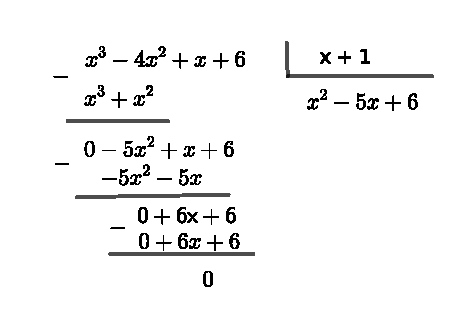
\includegraphics[width=8cm]{../Topicos/Figuras/polinomiosdivisao.pdf}
 \end{figure}
 
 note que o quociente da divisão é $q_1(x)= x^2 - 5x + 6$, e o resto desta divisão é $r(x)=0$ (zero). Como o resto é zero concluímos que $p_1(x)$ é divisível por $g_1(x)$. Portanto $p_1(x)= q_1(x)g_1(x)$, ou seja, $x^3-4x^2+x+6= (x^2-5x+6)(x+1)$.
 \end{exem}
 
 \begin{teo}
  Todo polinômio de grau $\geq 1$ em $K[x]$ pode ser expresso como um produto $p_1, \ldots, p_n$ de polinômios irredutíveis. Nesse produto, os polinômios $p_1, \ldots, p_n$ são determinados de modo único, a menos de um rearranjo, e a menos de eventuais fatores constantes não-nulos.   
 \end{teo}

